\section{Task Definition}
With a designated hard- and firmware extension for the LEGIC evaluation board EVB-6310, testing of the new UWB technology should be made possible for LEGIC customers. The evaluation board is based on the LEGIC security chip SM-6310, which includes a programmable ARM CORTEX and supports Bluetooth Low Energy, NFC and RFID. A possible arrangement of the extension (UWB-Board) and the evaluation board is shown in \cref{fig:constellation_HW} and subsequently referred to as UWB-Kit.

\begin{figure}[h!]
	\centering
	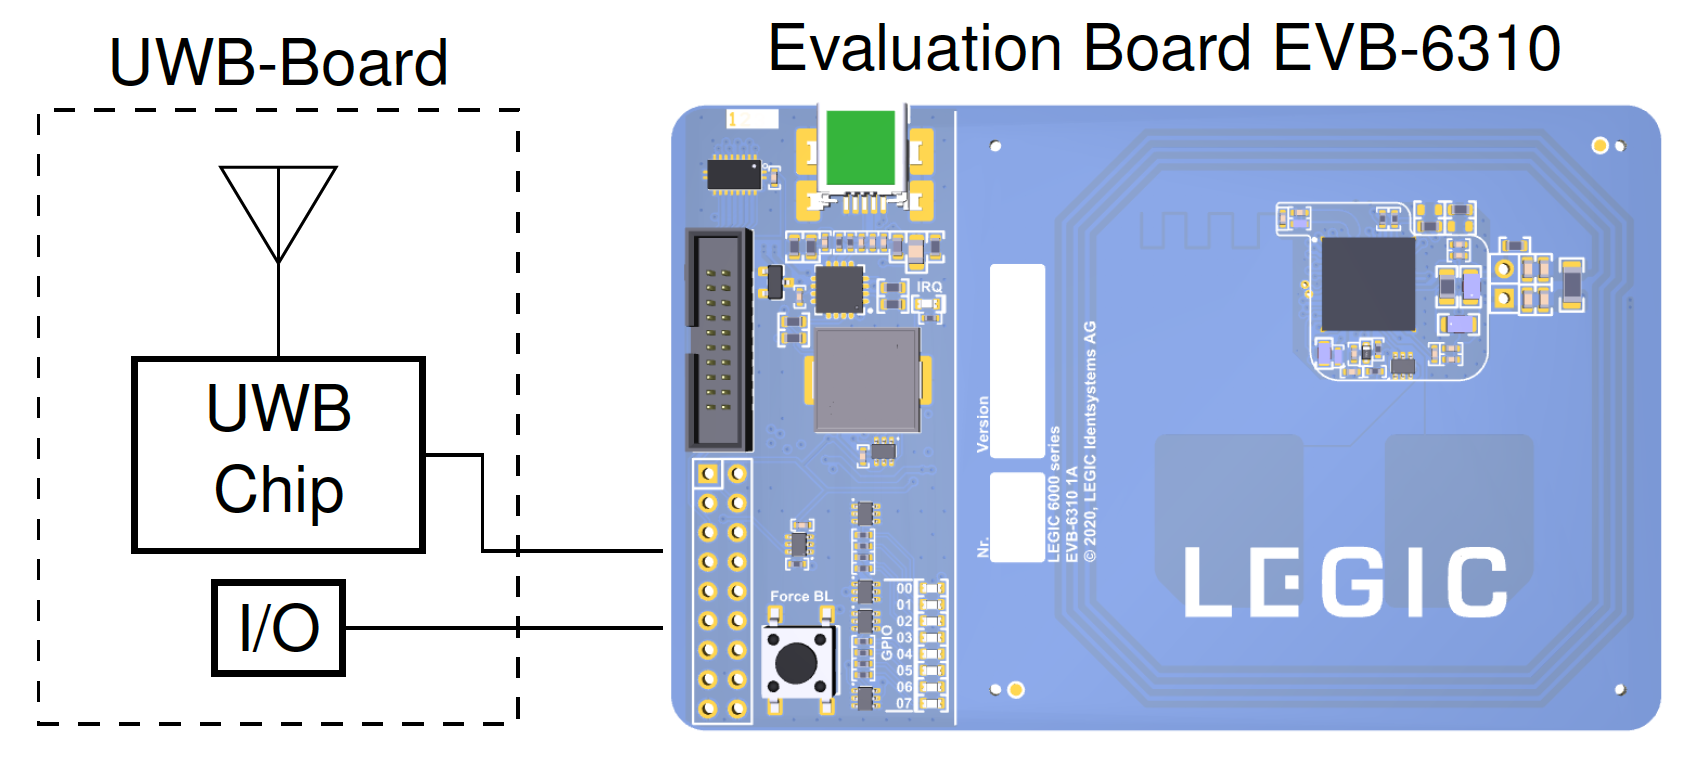
\includegraphics[width=11cm]{images/constellation_HW}
	\caption{Possible hardware arrangement}
	\vspace{-2ex}
	\caption*{\textbf{Source:} Original task definition}
	\label{fig:constellation_HW}
\end{figure}

To demonstrate general functionalities of UWB being
\begin{itemize}
	\item distance measuring between one or more UWB-Kits
	\item data communication between one or more UWB-Kits
	\item (optional) trilateration with three or more UWB-Kits
\end{itemize}

various use cases were defined in \cref{sec:use_cases}.

%With a designated hard- and firmware extension for the Legic Evaluation Board EVB-6310, testing of the new UWB-Technology should be made possible for LEGIC customers. The evaluation board is based on the LEGIC security chip SM-6310 which includes a customizable ARM CORTEX and supports Bluetooth Low Energy, NFC and RFID. %The UWB extension should preferably be realised with the silicon chip from the 3db Access AG and in the LRP-Mode.



%For the extension, UWB chips from 3db-Access should preferably be used. %, since they utilize the IEEE 802.15.4z standard.


%The existing Evaluation Board EVB-6310, based on the LEGIC security chip SM-6310, should be extended with UWB. This enables LEGIC customers to test the UWB-Technology. Today, the evaluation board implements 
